\documentclass[11pt,a4paper]{article}

\usepackage[spanish,es-tabla,es-noshorthands]{babel}
\usepackage[utf8]{inputenc}
\usepackage[T1]{fontenc}
\usepackage{lmodern}
\usepackage[margin=2.3cm]{geometry}
\usepackage{booktabs}
\usepackage{graphicx}
\usepackage{amsmath}
\usepackage[round]{natbib}
\usepackage{hyperref}
\usepackage{caption}

\hypersetup{
  colorlinks=true,
  linkcolor=black,
  citecolor=black,
  urlcolor=blue
}
\urlstyle{same}
\setlength{\parskip}{0.45em}
\setlength{\parindent}{0pt}
\renewcommand{\familydefault}{\sfdefault}

\title{Estimación del rendimiento de cebada\\con percepción remota y clima\\[0.4em]
\large Reto AgroCebada FIRA 2026}
\author{Equipo Los Vochos}
\date{Octubre de 2026}

\begin{document}
\maketitle
\begin{center}
\textit{Reporte técnico de la Etapa 1.}\\
Modelo de entrega: mezcla. Prototipo: dashboard web.
\end{center}
\vspace{0.6em}

% Meta: 400–550 palabras
\section{Introducción}

El sector agroalimentario enfrenta una mayor demanda de alimentos, el cambio climático y brechas de productividad e inclusión financiera. Los Fideicomisos Instituidos en Relación con la Agricultura (FIRA) atienden ese contexto con apoyos a la innovación tecnológica. Dentro del subcomponente Emprendedores Innovadores, el Reto AgroCebada 2026 pide un modelo analítico del rendimiento de parcelas de cebada en Hidalgo, Puebla y Tlaxcala, y una herramienta para consultar el resultado \citep{fira2026}.

La percepción remota describe el cultivo a lo largo del ciclo mediante índices de vegetación, y los rásteres climáticos aportan lluvia y temperatura. Esas fuentes ya existen. El problema es convertirlas en un estimado por parcela que resista un conjunto de evaluación cuyas etiquetas permanecen ocultas. El dataset oficial reúne 197 polígonos del ciclo abril–octubre de 2025. El rendimiento, en toneladas por hectárea, se observa en 138 parcelas. Las 59 restantes son el 30\,\% que el comité calificará. El equipo no usó esas etiquetas: entrenó solo con las 138 observadas y produjo un estimado para las 197.

Este reporte documenta el modelo de entrega, llamado mezcla, y el dashboard que lo consulta. La mezcla promedia dos predicciones. La primera es un ensamble de LightGBM, bosque aleatorio y red elástica \citep{ke2017,breiman2001,zou2005} entrenado con 121 variables de satélite, clima, topografía y ubicación. La segunda es un LightGBM que solo usa la longitud. Cada miembro del ensamble pesa un sexto y el modelo de longitud pesa un medio, de modo que la predicción final es el promedio simple del ensamble y del modelo de longitud.

La validación separa dos preguntas que no deben confundirse. La validación cruzada estratificada por municipio estima el error allí donde también están las parcelas ocultas: es la cifra que representa lo que se califica. Dejar un municipio completo fuera, esquema que aquí se llama LOMO, mide el deterioro cuando la zona es nueva dentro de la misma región. La distinción importa porque, en esta caja de unos 45 km, el rendimiento cambia de oeste a este y una parte de la señal es geográfica.

El escrito sigue la estructura pedida por las bases. Después de la justificación y los objetivos se describe la metodología, se reportan los resultados y se responden las tres preguntas guía. Un apartado vincula el estimado con la inclusión financiera del sector agropecuario. Cierran las conclusiones, la bibliografía y dos anexos: el trabajo del equipo y la declaración de uso de inteligencia artificial. Todas las cifras de desempeño provienen de los artefactos congelados que carga la API, no de una corrida paralela. El código, las instrucciones de ejecución y el enlace de la aplicación acompañan este documento para que el jurado pueda repetir el cálculo y consultar las parcelas.

% Meta: 100–200 palabras
\section{Justificación}

Anticipar el rendimiento por parcela, antes o al cierre del ciclo, cambia la calidad de la decisión. Un productor, un técnico o un intermediario financiero deja de depender solo del recuerdo de la zona y puede contrastar un estimado con el clima de la temporada y con el estado del cultivo visto desde satélite. En cebada de temporal, en el altiplano de Hidalgo, Puebla y Tlaxcala, esa información es escasa a escala de parcela y llega tarde si solo existe al momento de la cosecha.

El reto existe porque los datos públicos de percepción remota y de clima ya cubren la región, pero no están convertidos en una herramienta de consulta. Justifica el trabajo traducirlos a toneladas por hectárea, con un error medido y con límites explícitos, para que el número sirva de apoyo y no de promesa. Un estimado honesto, aunque imperfecto, es más útil para el crédito y la asistencia técnica que un modelo opaco que no dice dónde falla.

% Meta: ~200 palabras
\section{Objetivos}

El objetivo general es estimar el rendimiento de cebada (t/ha) en las 197 parcelas del reto y ofrecerlo en un dashboard que permita consultarlo parcela por parcela.

Los objetivos específicos son cuatro. Primero, construir una matriz de una fila por parcela a partir del dataset oficial, con índices de vegetación, clima mensual, topografía y ubicación, sin rellenar las 59 etiquetas ocultas. Segundo, comparar candidatos con la misma validación anidada: un ensamble de tres algoritmos, un modelo de solo longitud y la mezcla de ambos, y firmar como entrega el que equilibre el error donde se califica y el error en zona nueva. Tercero, interpretar el modelo firmado lo suficiente para responder qué índice, qué variable climática y qué bloque de variables aportan más, declarando que la explicación SHAP no cubre la mezcla completa. Cuarto, servir las predicciones congeladas mediante una API de solo lectura y un tablero con mapa, ficha, métricas, hallazgos y simulador, documentado para ejecutarse desde el repositorio. El objetivo no es maximizar un indicador a costa de opacidad: el error, el esquema de validación y los límites de transferencia deben poder leerse junto con el número de cada parcela. También queda escrito cómo regenerar los artefactos.

% Meta: 600–700 palabras
\section{Metodología}

\subsection{Datos y unidad de análisis}

La unidad es la parcela. El archivo oficial aporta el polígono, el identificador \texttt{AGC}, el municipio y, solo en el 70\,\% de los casos, el rendimiento del ciclo abril–octubre de 2025. Se unió cada polígono con series de índices del conjunto Básico (Sentinel-2 y Landsat) y del conjunto PRO (Planet), con lluvia y temperatura mensuales y con elevación y pendiente \citep{esa_s2,huete2002}. Las fechas se leyeron en formato día/mes/año. La lluvia y la temperatura llegan en GeoTIFF mensuales de unos 5 km de lado. La elevación y la pendiente se reproyectaron antes de la estadística zonal. Un rendimiento vacío se dejó vacío: sustituirlo por cero habría fabricado una cosecha nula.

El equipo revisó dos fuentes públicas adicionales: edafología del INEGI y propiedades de SoilGrids, en particular el nitrógeno \citep{inegi,poggio2021}. Sirvieron para un carril paralelo de experimentos. No entran en el modelo de entrega. Una prueba pareada, descrita más adelante, mostró que no mejoran el error bajo un criterio fijado de antemano.

\subsection{Variables}

De la serie satelital no se usó solo el pico del índice. El análisis exploratorio indicó que el máximo casi no separa parcelas, y que sí aportan la velocidad de verdeo, la de senescencia y la integral de la temporada. El modelo de entrega usa 121 variables: dinámicas de índices (NDVI, EVI, LAI, NDWI, NDDI y otros del conjunto oficial), lluvia y temperaturas mensuales del ciclo, elevación, pendiente y coordenadas. El modelo de solo longitud usa una variable, \texttt{lon}.

\subsection{Candidatos y entrenamiento}

Se compararon tres predictores con las mismas 138 parcelas etiquetadas. El ensamble promedia tres algoritmos: LightGBM, bosque aleatorio y red elástica \citep{ke2017,breiman2001,zou2005,pedregosa2011}. Los tres ven las 121 variables. Un imputador de mediana es común; el escalador solo lo usa la red elástica. El segundo candidato es un LightGBM de longitud. La mezcla es el promedio de la predicción del ensamble y la del modelo de longitud. En pesos, cada miembro del ensamble aporta un sexto y la longitud aporta un medio.

Los hiperparámetros del ensamble se eligieron con Optuna anidado: la búsqueda solo ve el pliegue de entrenamiento, no el de prueba \citep{akiba2019}. Así se evita premiar una configuración que ya vio la parcela que se evalúa. Antes de firmar la mezcla, un barrido de modelos clásicos sobre más de mil combinaciones de features (el superciclo) señaló a la longitud como señal fuerte. Ese barrido no sustituyó al pipeline: aportó la hipótesis que luego se probó dentro de la misma validación.

\subsection{Validación}

Hay dos esquemas. El primero es una validación cruzada anidada estratificada por municipio, con cinco pliegues y tres repeticiones. Como las 59 parcelas ocultas están en los mismos municipios que las 138 observadas, este error es el que representa la calificación. El segundo, LOMO, deja fuera un municipio completo en cada ronda y mide el desempeño en una zona no vista de la región. Diferencias menores a 0.010 t/ha se trataron como ruido de la validación, no como mejora.

El criterio para cambiar el modelo de entrega se fijó antes de la prueba del ganador del superciclo. Un candidato solo reemplazaría a la mezcla si bajaba el RMSE estratificado al menos 0.010 t/ha, no empeoraba el LOMO y el intervalo bootstrap del 95\,\% de la diferencia por parcela excluía el cero. Ninguna variante, con o sin nitrógeno y edafología, cumplió las tres condiciones. Por eso la entrega no incorpora datos externos.

\subsection{Explicación y producto}

Las importancias se calcularon con SHAP sobre el LightGBM del ensamble \citep{lundberg2017}. Esa pieza pesa un sexto de la mezcla. La cascada de una parcela explica esa pieza, no el promedio final: el modelo de longitud y los otros dos miembros no entran en el valor SHAP. El reporte y el dashboard lo dicen de forma explícita.

En operación el pipeline exporta artefactos de unos 2 MB. Django los carga al arrancar y no reentrena. El dashboard consulta mapa, ficha, métricas, hallazgos y simulador; está en Vercel y la API en Render. El simulador mueve el clima dentro del rango observado y, como solo el ensamble reacciona, el efecto sale a la mitad. El artefacto en línea cuenta 122 variables en la mezcla; aquí son 121, porque la longitud ya va en esas columnas.

% Meta: ~800 palabras
\section{Resultados y discusión}

\subsection{Desempeño de la mezcla}

La tabla~\ref{tab:candidatos} resume la comparación anidada. Donde se califica, el ensamble y la mezcla empatan en RMSE (0.508 t/ha) y en $R^{2}$ (0.64). La mezcla tiene mejor MAE (0.354 frente a 0.362) y un sesgo de +0.005 t/ha. Predecir el promedio de las parcelas de entrenamiento da un RMSE de 0.846: la mezcla recorta ese error en cerca de un 40\,\%. El modelo de solo longitud queda cerca en la estratificada (0.525) y es el mejor en LOMO (0.539), lo que confirma que la geografía carga mucha señal. El ensamble, en cambio, se degrada al sacar un municipio (RMSE 0.722, sesgo $-0.102$). La mezcla queda en medio (0.595, sesgo $-0.013$): no pierde donde se califica y recorta casi la mitad de la caída del ensamble en zona nueva. Por ese equilibrio se firmó como entrega. La figura~\ref{fig:dispersion} muestra las 138 predicciones fuera de muestra frente al valor observado; la figura~\ref{fig:residuales}, los residuales.

\begin{table}[ht]
\centering
\caption{Tres candidatos, mismas 138 parcelas. RMSE, MAE y sesgo en t/ha.}
\label{tab:candidatos}
\small
\begin{tabular}{lrrrrrr}
\toprule
 & \multicolumn{3}{c}{Estratificada} & \multicolumn{2}{c}{LOMO} \\
\cmidrule(lr){2-4}\cmidrule(lr){5-6}
Candidato & RMSE & MAE & $R^{2}$ & RMSE & Sesgo \\
\midrule
Ensamble (121 var.) & 0.508 & 0.362 & 0.64 & 0.722 & $-0.102$ \\
Solo longitud & 0.525 & 0.364 & 0.62 & 0.539 & +0.077 \\
Mezcla (entrega) & 0.508 & 0.354 & 0.64 & 0.595 & $-0.013$ \\
\bottomrule
\end{tabular}
\end{table}

\begin{figure}[ht]
\centering
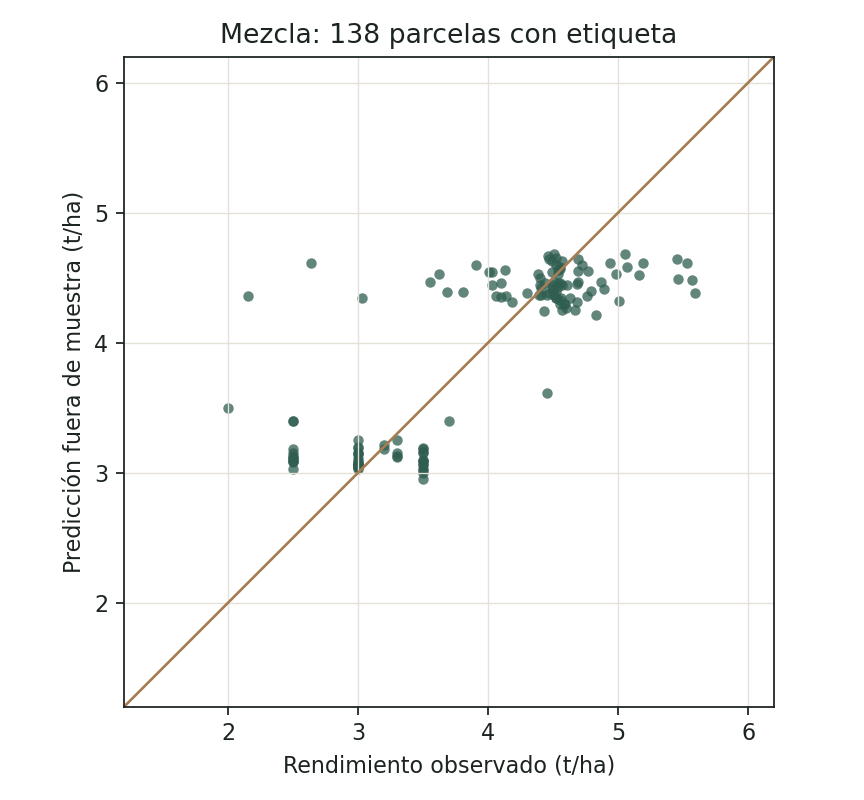
\includegraphics[width=0.72\textwidth]{figuras/dispersion.png}
\caption{Observado contra predicción fuera de muestra de la mezcla.}
\label{fig:dispersion}
\end{figure}

\begin{figure}[ht]
\centering
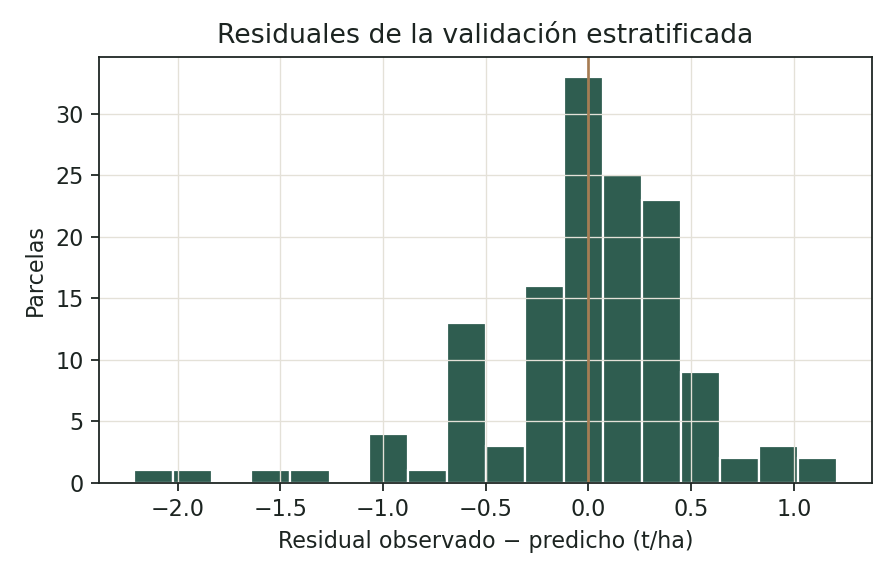
\includegraphics[width=0.78\textwidth]{figuras/residuales.png}
\caption{Distribución de residuales de la validación estratificada.}
\label{fig:residuales}
\end{figure}

La prueba del ganador del superciclo, hecha con los mismos pliegues, no cambió la firma. Ese LightGBM, de 13 variables y con nitrógeno de SoilGrids más edafología, obtuvo un RMSE estratificado de 0.582 t/ha, peor que la mezcla. Con Optuna anidado bajó a 0.547 y, mezclado con el ensamble, a 0.520. En ningún caso se cumplieron a la vez la mejora de 0.010 t/ha, un LOMO no peor y un intervalo bootstrap por debajo de cero. Los datos externos no compraron precisión en el conjunto que se califica.

Al dejar un municipio fuera, el error de la mezcla no es uniforme (figura~\ref{fig:lomo}). Con al menos cinco parcelas, Almoloya queda en 0.28 t/ha ($n=10$), Cuautepec de Hinojosa en 0.32 ($n=5$), Calpulalpan en 0.44 ($n=30$), Chignahuapan en 0.61 ($n=71$) y Singuilucan en 0.90 ($n=16$). Chignahuapan concentra la mitad de la muestra; Singuilucan es el punto débil. El agregado LOMO de 0.595 es un promedio exigente, no un error típico de cada municipio. La figura omite municipios de menos de cinco parcelas.

\begin{figure}[ht]
\centering
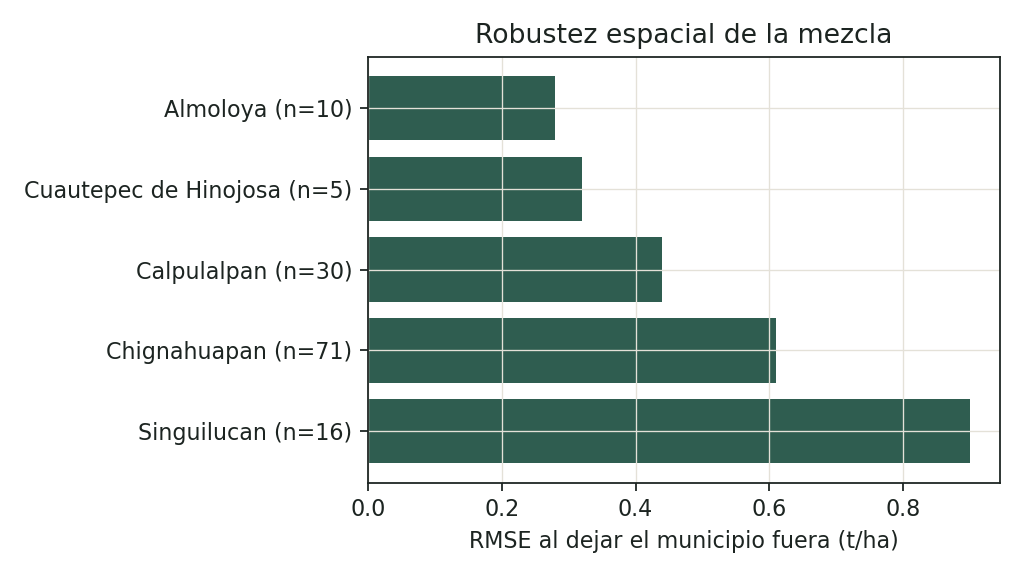
\includegraphics[width=0.82\textwidth]{figuras/lomo_municipio.png}
\caption{RMSE de la mezcla al excluir cada municipio con al menos cinco parcelas.}
\label{fig:lomo}
\end{figure}

\subsection{Preguntas guía}

Las respuestas usan el valor absoluto medio de SHAP del LightGBM del ensamble. No describen la mezcla completa.

\textit{¿Qué índice pesa más?} Al sumar las contribuciones de las variables derivadas de cada índice, el mayor es el NDVI (0.081 t/ha), seguido del NDDI (0.072) y del LAI (0.050). Dentro del NDVI, la velocidad de senescencia (0.049) supera al valor máximo (0.002). El pico de verdor casi no discrimina; la dinámica del ciclo sí. La figura~\ref{fig:shap} agrupa esas familias.

\textit{¿Qué variable climática pesa más?} La lluvia de mayo (\texttt{prec\_mm\_m05}) concentra 0.268 t/ha de $|$SHAP$|$, muy por encima de la lluvia de abril (0.047), la temperatura máxima de abril (0.026) y la mínima de abril (0.021). La familia climática suma 0.381, la mayor de todas. Ese peso no demuestra que la lluvia de mayo cause el rendimiento: el píxel climático mide unos 5 km y puede estar actuando como indicador de zona, del mismo modo que la longitud.

\textit{¿Qué combinación funciona mejor?} La ablación, con el mismo esquema estratificado, ordena los bloques así: solo clima, 0.507 t/ha (16 variables); todas las variables, 0.508 (121); clima más satélite, 0.512 (99); topografía y ubicación, 0.514 (16); clima y ubicación, 0.523 (32); solo satélite, 0.613 (83). El mejor bloque puntual es el clima. La diferencia con el modelo completo es de 0.001 t/ha, dentro del ruido de 0.010. El satélite solo, sin clima, es claramente peor. La mezcla se quedó con las 121 variables porque el empate no justifica tirar el satélite, que sí aporta en la ficha y en la lectura agronómica, y porque el criterio de entrega miraba también el LOMO, no solo esta ablación. La figura~\ref{fig:ablacion} muestra la comparación.

\begin{figure}[ht]
\centering
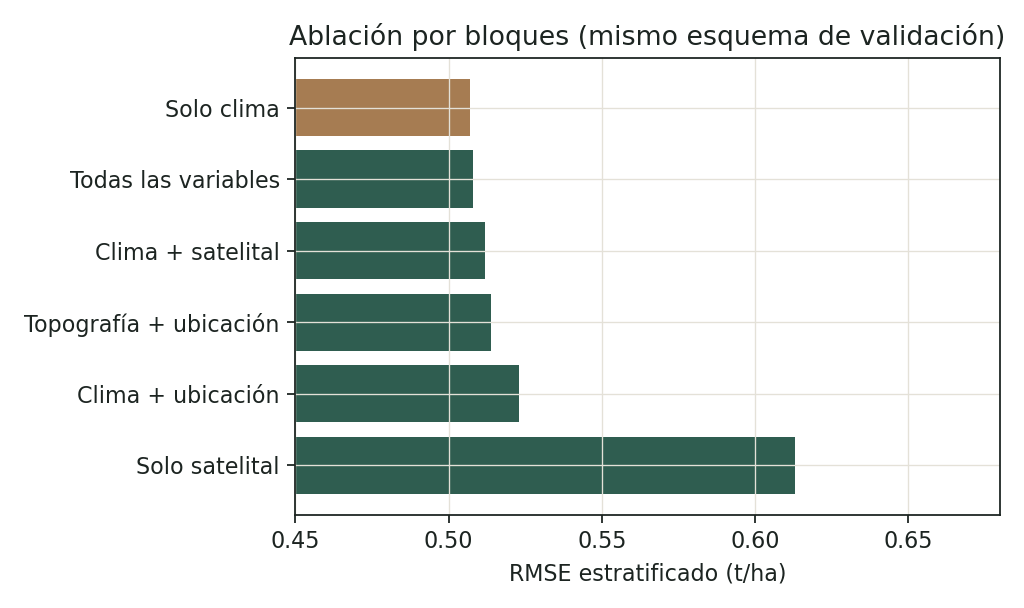
\includegraphics[width=0.86\textwidth]{figuras/ablacion.png}
\caption{RMSE estratificado por bloque de variables.}
\label{fig:ablacion}
\end{figure}

\begin{figure}[ht]
\centering
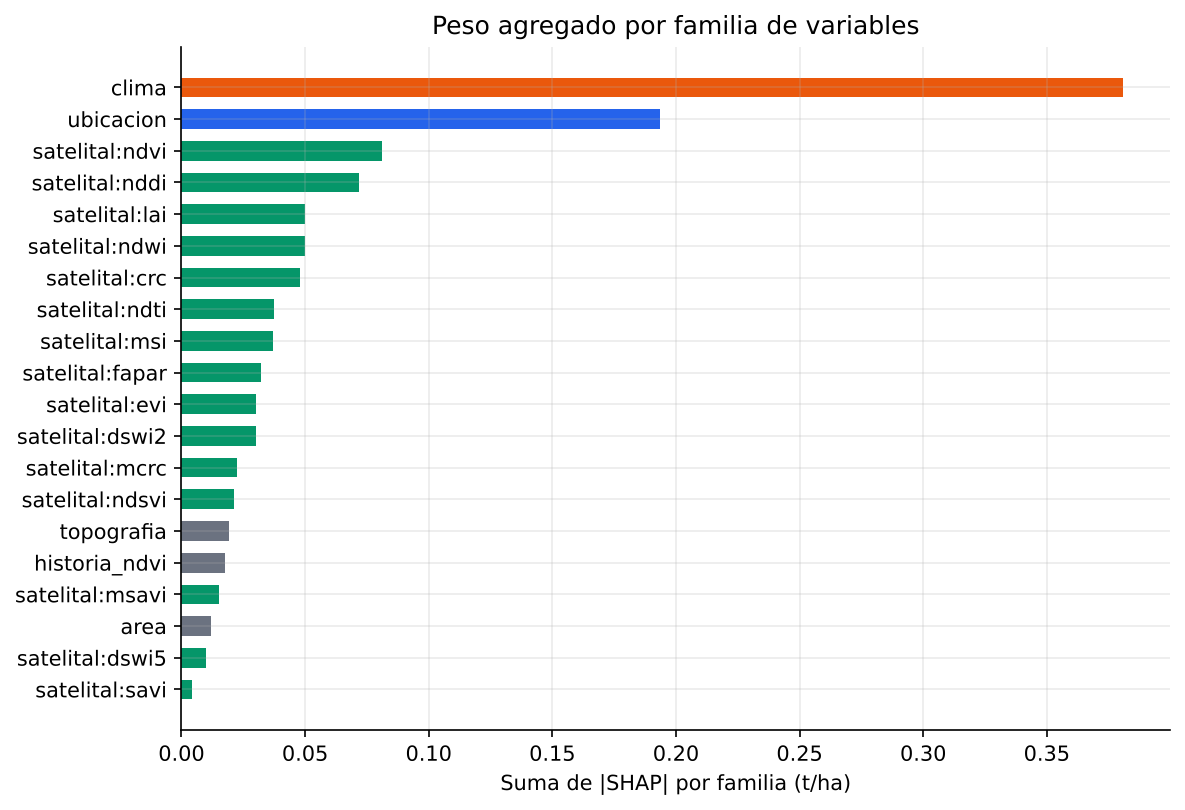
\includegraphics[width=0.92\textwidth]{figuras/fig_shap_familias.png}
\caption{Contribución $|$SHAP$|$ por familia en el LightGBM del ensamble (peso 1/6 de la mezcla).}
\label{fig:shap}
\end{figure}

\subsection{Límites}

Las 59 predicciones de entrega están calculadas y se consultan en el dashboard, pero este reporte no les asigna un error: la etiqueta la resguarda el comité. Publicar un RMSE sobre ellas sería inventar la calificación.

El modelo vio una sola temporada. Fuera de esta región la longitud no es transferible: habría que reentrenar con rendimientos locales. En el simulador, el efecto climático aparece atenuado a la mitad porque la longitud no se mueve. En Tlaxcala el rendimiento observado toma pocos valores, lo que parece una estimación por zona más que una medición parcela a parcela. La herramienta apoya la consulta; no sustituye la evaluación crediticia ni una visita de campo.

% Meta: ~300 palabras
\section{Uso de la ciencia de datos en la inclusión financiera del sector agro}

Las Reglas de Operación de los apoyos al sector agropecuario buscan ampliar el acceso al financiamiento formal y mejorar la productividad de las unidades rurales \citep{fira2025reglas}. Un obstáculo es la información: quien evalúa un crédito suele conocer la zona mejor que la parcela, y el rendimiento anterior llega cuando la decisión ya se tomó. Un estimado por polígono, construido con datos públicos de satélite y clima, no reemplaza el expediente ni la visita, pero sí adelanta una magnitud en toneladas por hectárea y un intervalo de error conocido.

En la práctica, el dashboard permite tres usos alineados con esa política. El primero es de tamiz: ordenar parcelas de una zona por el estimado y por el residual histórico, para concentrar la asistencia técnica donde el modelo y el clima de la temporada se separan. El segundo es de conversación con el productor: la ficha muestra el número, las variables que más empujan esa parcela y la aclaración de que la explicación no cubre toda la mezcla. El tercero es de límite institucional: el RMSE de 0.508 t/ha donde se califica, y el deterioro en Singuilucan o al salir del municipio, indican hasta dónde el dato puede pesar en una resolución de crédito. Usarlo como si fuera un aforo medido reproduciría la exclusión por otro camino, el de un modelo opaco.

La viabilidad es modesta. No hace falta una red de sensores en la parcela: hacen falta el polígono, el ciclo y no extrapolar a otra región ni a otro año sin reentrenar. El código y los artefactos permiten repetir la consulta. Si el estimado se usara en operación, el siguiente paso sería contrastarlo con las etiquetas ocultas y, sobre todo, con más de una temporada.

% Meta: ~400 palabras
\section{Conclusiones}

Se entrega un estimado de rendimiento de cebada para las 197 parcelas del Reto AgroCebada 2026 y un dashboard para consultarlo. El modelo firmado es la mezcla: el promedio de un ensamble (LightGBM, bosque aleatorio y red elástica, 121 variables) y un LightGBM de solo longitud. En la validación estratificada por municipio, que representa a las 59 parcelas ocultas, el RMSE es 0.508 t/ha, el MAE 0.354 y el $R^{2}$ 0.64, frente a 0.846 de predecir el promedio. En zona nueva (LOMO) el RMSE sube a 0.595, con un sesgo cercano a cero, y queda entre el ensamble, que se cae, y la longitud, que generaliza mejor pero explica menos del cultivo.

Esa elección no fue el ganador automático de un barrido amplio. El superciclo y la prueba de datos externos (INEGI y SoilGrids) se evaluaron con un criterio escrito antes de ver el resultado. No bajaron el error estratificado en al menos 0.010 t/ha sin empeorar el LOMO. La longitud sí se incorporó, como la mitad de la mezcla, porque en esta región el gradiente oeste–este es real y medible.

Las preguntas guía tienen respuesta acotada. El índice de mayor contribución SHAP es el NDVI, sobre todo por la senescencia y no por el pico. La variable climática de mayor peso es la lluvia de mayo. El bloque de menor RMSE es el clima, empatado en la práctica con el modelo completo; el satélite solo no basta. Esas lecturas describen un sexto de la mezcla, el LightGBM del ensamble, y la lluvia de mayo puede ser proxy de zona.

Los límites son parte del resultado. Hay una sola temporada, el modelo no debe salir de estos municipios sin datos nuevos, y el simulador atenúa a la mitad cualquier cambio de clima. El producto es una herramienta de apoyo a la consulta y, en el margen, a la conversación de crédito y asistencia técnica. No es un aforo ni una resolución de financiamiento.

El dashboard ya muestra el mapa, la ficha, las métricas y el simulador. Queda abierto repetir el ciclo en otras temporadas, publicar el contraste contra las 59 etiquetas cuando el comité las libere y volver a probar datos de suelo solo si pasan el mismo criterio. El código de la API y del dashboard está publicado, con instrucciones para correrlo en local, de modo que esa revisión no exija reconstruir el trabajo desde cero.


\bibliographystyle{plainnat}
\bibliography{referencias}

\appendix
% Máximo 2 cuartillas. Trabajo del equipo en bloque; sin desglose por persona.
\section{Trabajo del equipo}

El equipo construyó el entregable de punta a punta sobre el dataset oficial. Revisó la calidad de los datos FIRA y, en carriles aparte, la edafología del INEGI y SoilGrids. Congeló una despensa de entrenamiento y comparó cientos de combinaciones de variables con modelos clásicos. Con esa evidencia incorporó la longitud a un pipeline reproducible, comparó ensamble, ubicación y mezcla bajo validación anidada, y descartó sustituir la mezcla por el ganador del barrido o por datos externos. Exportó artefactos congelados, los sirvió con una API de solo lectura y los consultó en un dashboard con mapa, ficha, métricas, hallazgos y simulador. Publicó la API y el dashboard en sus propios repositorios y dejó en este las instrucciones para ejecutarlos en local.

\section{Declaración de uso de inteligencia artificial}

El uso de inteligencia artificial está permitido si se indica dónde se usó y se anexan los prompts \citep{fira2026}. El equipo la usó como apoyo de programación, redacción técnica y revisión de código. Las decisiones de modelo (firmar la mezcla, el umbral de 0.010 t/ha, no usar etiquetas ocultas) las fijó el equipo y quedaron escritas antes de aceptar un resultado.

\begin{table}[ht]
\centering
\caption{Dónde se usó inteligencia artificial. El detalle de cada prompt está en \texttt{PROMPTS.md} del repositorio.}
\label{tab:ia}
\small
\begin{tabular}{p{3.3cm}p{3.4cm}p{6.6cm}}
\toprule
Área & Herramienta & Qué se le pidió (representativo) \\
\midrule
Análisis y despensa & Agentes en Cursor & Documentar el dataset, congelar la despensa y comparar carriles FIRA, INEGI y SoilGrids. \\
Modelos & Agentes en Cursor & Diseñar el superciclo, interpretar al ganador y probarlo dentro del pipeline de la mezcla. \\
Integración & Agentes en Cursor & Unir API y dashboard al repositorio, reubicar el pipeline y corregir la documentación de ejecución. \\
API y dashboard & Claude Code & Implementar el backend de artefactos y el tablero Angular. Las sesiones quedaron referenciadas en los commits (\texttt{Co-Authored-By}); la transcripción completa está pendiente de incorporarse a \texttt{PROMPTS.md}. \\
Este reporte & Agentes en Cursor & Redactar el LaTeX a partir de las cifras de los artefactos y el guion del video. \\
\bottomrule
\end{tabular}
\end{table}

\noindent No se usó inteligencia artificial para inventar rendimientos, para imputar las 59 etiquetas ocultas ni para alterar el dataset oficial. Los prompts de las sesiones de análisis, modelos, integración y de este reporte están en \texttt{PROMPTS.md}. Los de la construcción original de la API y del dashboard se identifican por el enlace de sesión en el historial de git y quedan como complemento pendiente del equipo.


\end{document}
